\iffalse
\let\negmedspace\undefined
\let\negthickspace\undefined
\documentclass[journal,12pt,twocolumn]{IEEEtran}
\usepackage{cite}
\usepackage{amsmath,amssymb,amsfonts,amsthm}
\usepackage{algorithmic}
\usepackage{graphicx}
\usepackage{textcomp}
\usepackage{xcolor}
\usepackage{txfonts}
\usepackage{listings}
\usepackage{enumitem}
\usepackage{mathtools}
\usepackage{gensymb}
\usepackage{comment}
\usepackage[breaklinks=true]{hyperref}
\usepackage{tkz-euclide}
\usepackage{listings}
\usepackage{gvv}
\def\inputGnumericTable{}
\usepackage[latin1]{inputenc}
\usepackage{color}
\usepackage{array}
\usepackage{longtable}
\usepackage{calc}
\usepackage{multirow}
\usepackage{hhline}
\usepackage{ifthen}
\usepackage{lscape}

\newtheorem{theorem}{Theorem}[section]
\newtheorem{problem}{Problem}
\newtheorem{proposition}{Proposition}[section]
\newtheorem{lemma}{Lemma}[section]
\newtheorem{corollary}[theorem]{Corollary}
\newtheorem{example}{Example}[section]
\newtheorem{definition}[problem]{Definition}
\newcommand{\BEQA}{\begin{eqnarray}}
\newcommand{\EEQA}{\end{eqnarray}}
\newcommand{\define}{\stackrel{\triangle}{=}}
\theoremstyle{remark}
\newtheorem{rem}{Remark}
\begin{document}

\bibliographystyle{IEEEtran}
\vspace{3cm}
	\title{NCERT Maths 10.5.3 Q14}
	\author{EE23BTECH11201 - ABBURI TANUSHA$^{*}$% <-this % stops a space
	}
\maketitle
\newpage
\bigskip

\renewcommand{\thefigure}{\theenumi}
\renewcommand{\thetable}{\theenumi}

\vspace{3cm}
\maketitle
\textbf{Question:} 
Find the sum of odd numbers between $0$ and $50$.

\solution
\fi
\begin{table}[h!]
	\centering
	 \resizebox{6cm}{!}{
	 	
\begin{tabular}{|c|c|c|}
	\hline
	\textbf{Symbol} & \textbf{Value} & \textbf{Description} \\[6pt]
	\hline
	$x(0)$ & $1$ & first term of AP \\[6pt]
	\hline
	$d$ & $2$ & common difference \\[6pt]
	\hline
	$x(n)$ & $(1+2n)u(n)$ & $n$-th term of AP \\[6pt]
	\hline
\end{tabular}


	 	}
	 	\caption{Given Parameters}
	 	\label{tab:ansh_tabel}
 \end{table}

Last term of the given sequence is 49.
\begin{align}
 x(n) &= (2n+1)u(n) \\
 \therefore ( 2n +1 ) &= 49 \\
\implies n &= 24 
\end{align}
Applying Z transform
From equation \eqref{eq:11.9.5.26.2}:
\begin{align}
   X(z) &= \frac{1+z^{-1}}{(1-z^{-1})^2},  \quad \abs{z} > \abs{1}  
\end{align}
For AP, the sum of first n+1 terms can be written as 
\begin{align}
y(n)&=x(n)*u(n) \\
Y(z) &= X(z)U(z)\\
 &=\frac{1}{(1-z^{-1})^2} + \frac{2z^{-1}}{(1-z^{-1})^3}, \quad \abs{z} > \abs{1} 
\end{align}
Using contour integration to find inverse Z transform
\begin{align}
y(n) &= \frac{1}{2\pi j} \oint_C Y(z) z^{n-1} dz\\
y(24) &= \frac{1}{2\pi j}\int Y(z) z^{23} dz \\
 &= \frac{1}{2\pi j}\int \frac{1.z^{25}}{(z-1)^{2}} dz - \frac{1}{2\pi j}\int \frac{2.z^{25}}{(z-1)^{3}} dz\\
 \because R&=\frac{1}{\brak {m-1}!}\lim\limits_{z\to a}\frac{d^{m-1}}{dz^{m-1}}\brak {{(z-a)}^{m}f\brak z}
 \end{align}
 For R1 , $m = 2$ , where m corresponds to number of repeated poles \\
 \begin{align}
 R_1 &=\frac{1}{1!}\lim\limits_{z\to 1}\frac{d}{dz}\brak {(z-1)^2.\frac{1.z^{25}}{(z-1)^{2}}}\\
 &= 25
 \end{align}
 For R2 , $m = 3$ \\
 \begin{align}
 R_2 &=\frac{1}{2!}\lim\limits_{z\to 1}\frac{d^2}{dz^2}\brak {(z-1)^3.\frac{2.z^{25}}{(z-1)^{3}}}\\
 &= 600\\
 \implies y(24) &= R_1 + R_2 \\
&= 625
\end{align}

\begin{figure}[h!]
\centering
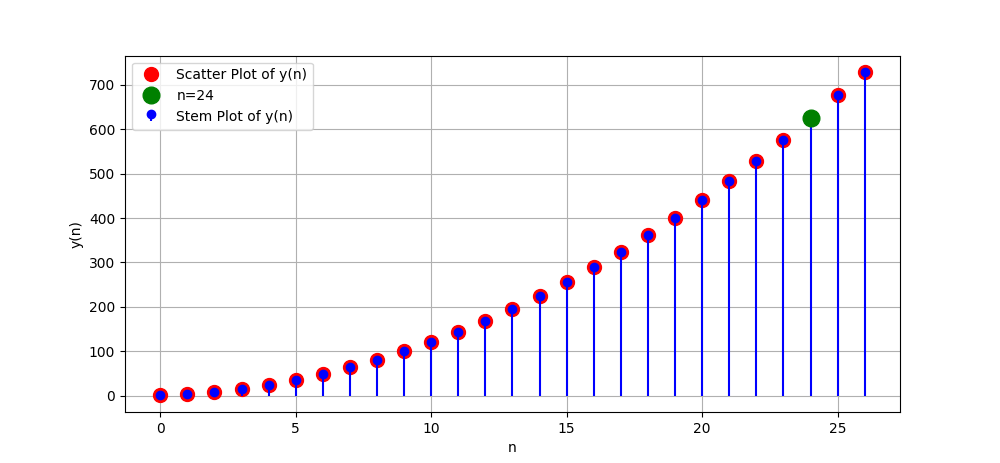
\includegraphics[width=\columnwidth]{ncert-maths/10/5/3/14/figs/stem_plot.png}
\label{fig:tans_plott}
\caption{Combination of stem and scatter plot of y(n)}
\end{figure}
%\end{document}

 
